% !TeX root = ../../main.tex

\chapter{Konzept}
In diesem Abschnitt wird kurz unser Konzept für die Umsetzung von Sfm erläutert. 
Insbesondere wird dabei erläutert, was in den einzelnen Schritten durchgeführt wird, und warum diese Schritte notwendig sind.
Details zur Implementierung werden in Kapitel~\ref{sec:implementation} beschrieben.

Das Konzept ist eine einfache Pipeline von vier Prozessen, durch die Bildpunkte rekonstruiert werden.
Die Pipeline ist in Abb.~\ref{fig:concept-pipeline} dargestellt.
Der erste Prozess \emph{Kalibrierung} bestimmt die Parameter der Kamera, mit der die Bilder zur Rekonstruktion aufgenommen wurden.
Dieser Schritt ist nötig, da bei der Rekonstruktion die Kalibrierungsmatrix K benötigt wird.
Diese Matrix enthält Informationen über die Brennweite der Kamera und der Position des Hauptpunkts im Bild.
Des Weiteren wird bei der Kalibrierung auch die Verzerrungkoeffizienten der Linse der Kamera bestimmt. %TODO Koeffizienten in Kalibrierungskapitel erläutern
Damit kann die Verzerrung in den Bildern reduziert werden, was zu genaueren Ergebnissen bei der Rekonstruierung führt.% TODO: muss belegt werden. gff im Kapitel Kalibrierung beschreiben 
Die Kalibrierung wird mit Hilfe eines Schachbrettmusters durchgeführt, weil *Insert befriedigende Begründug*.
Daher müssen zusätzliche Bilder für die Kalibrierung vom Nutzer bereitgestellt werden.
Da ggf.\ die Kalibrierung zeitaufwendig sein kann, wird die Möglichkeit bereitgestellt, die Kameraparameter zu exportieren.
Diese Datei kann dann geladen werden, so dass keine Kalibrierung durchgeführt werden muss. 
Es wird jedoch keine weiteren Features für die Verwaltung der Kalibrierungen angeboten.
Der Nutzer ist als selbst dafür verantwortlich zu wissen, welche Datei zu welcher Kamera gehört und welche Kalibrierungsdatei für die Pipeline benötigt wird. 








\begin{figure}
    \centering
    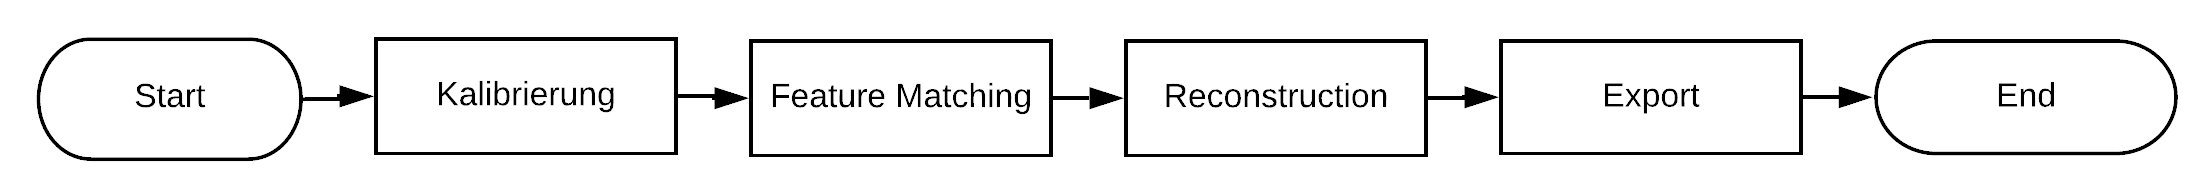
\includegraphics{src/img/konzept-pipeline-horizontal.png}
    \caption{Rekonstruktierungspipline des Konzepts}
    \label{fig:concept-pipeline}
\end{figure}
